
% SIAM Article Template
\documentclass[review,onefignum,onetabnum]{siamart171218}

% Information that is shared between the article and the supplement
% (title and author information, macros, packages, etc.) goes into
% ex_shared.tex. If there is no supplement, this file can be included
% directly.

% SIAM Shared Information Template
% This is information that is shared between the main document and any
% supplement. If no supplement is required, then this information can
% be included directly in the main document.


% Packages and macros go here
\usepackage{lipsum}
\usepackage{amsfonts}
\usepackage{amssymb}
\usepackage{amsmath}
\DeclareMathOperator*{\argmax}{arg\,max}
\DeclareMathOperator*{\argmin}{arg\,min}

\usepackage{graphicx}
\usepackage{epstopdf}
\usepackage{algorithmic}
\ifpdf
  \DeclareGraphicsExtensions{.eps,.pdf,.png,.jpg}
\else
  \DeclareGraphicsExtensions{.eps}
\fi


\newcommand{\floor}[1]{\left\lfloor #1 \right\rfloor}
\newcommand{\ceil}[1]{\left\lceil #1 \right\rceil}
\newcommand{\stcomp}[1]{{#1}^\complement}


% Add a serial/Oxford comma by default.
\newcommand{\creflastconjunction}{, and~}

% Used for creating new theorem and remark environments
\newsiamremark{remark}{Remark}
\newsiamremark{hypothesis}{Hypothesis}
\crefname{hypothesis}{Hypothesis}{Hypotheses}
\newsiamthm{claim}{Claim}

% Sets running headers as well as PDF title and authors
\headers{The Horse Race Problem}{P. Cotton}

% Title. If the supplement option is on, then "Supplementary Material"
% is automatically inserted before the title.
\title{Inferring Relative Ability from Winning \\ Probability
in Multi-Entrant Contests\thanks{Submitted to the editors July 2019.
}}

% Authors: full names plus addresses.
\author{Peter Cotton\thanks{Intech Investments
  (\email{peter.cotton@intechinvestments.com}). We thank reviewers for helpful feedback.}
  }

\usepackage{amsopn}
\DeclareMathOperator{\diag}{diag}


%% Added on Overleaf: enabling xr
\makeatletter
\newcommand*{\addFileDependency}[1]{% argument=file name and extension
  \typeout{(#1)}% latexmk will find this if $recorder=0 (however, in that case, it will ignore #1 if it is a .aux or .pdf file etc and it exists! if it doesn't exist, it will appear in the list of dependents regardless)
  \@addtofilelist{#1}% if you want it to appear in \listfiles, not really necessary and latexmk doesn't use this
  \IfFileExists{#1}{}{\typeout{No file #1.}}% latexmk will find this message if #1 doesn't exist (yet)
}
\makeatother

\newcommand*{\myexternaldocument}[1]{%
    \externaldocument{#1}%
    \addFileDependency{#1.tex}%
    \addFileDependency{#1.aux}%
}
%%% END HELPER CODE
%%% Local Variables: 
%%% mode:latex
%%% TeX-master: "ex_article"
%%% End: 


% Optional PDF information
\ifpdf
\hypersetup{
  pdftitle={Inferring Relative Ability from Winning Probability
   in Multi-Entrant Contests},
  pdfauthor={Peter Cotton}
}
\fi

% The next statement enables references to information in the
% supplement. See the xr-hyperref package for details.

%% Use \myexternaldocument on Overleaf
\myexternaldocument{ex_supplement}

% FundRef data to be entered by SIAM
%<funding-group>
%<award-group>
%<funding-source>
%<named-content content-type="funder-name"> 
%</named-content> 
%<named-content content-type="funder-identifier"> 
%</named-content>
%</funding-source>
%<award-id> </award-id>
%</award-group>
%</funding-group>

\begin{document}

\maketitle

% REQUIRED
\begin{abstract}
We provide a fast and scalable numerical algorithm for inferring the distributions of participant scores in a multi-party contest, under the assumption that each participant's score distribution is a translation of every other's. We term this the horse race problem, as the solution provides one way of assigning coherent probabilities to all outcomes, and pricing arbitrarily complex horseracing wagers. However the algorithm may also find use anywhere winning probabilities are apparent, such as with e-commerce product placement, in web search, or, as we show, in addressing a fundamental problem of trade: who to call, based on market share statistics and inquiry cost.    
\end{abstract}

% REQUIRED
\begin{keywords}
  order statistics, rank statistics, trifecta, exacta, quinella, baseball pythagorean theorem, inverse problems, horse racing, handicapping, asset pricing, coherent probability, risk neutral pricing, web search
\end{keywords}

% REQUIRED
\begin{AMS}
  62P20
\end{AMS}


\section{The discrete horse race problem} 
\label{sec:problem}

In this section we define the discrete horse race problem, for which we present a solution in Section \ref{sec:solution}. This finds use in some horseracing related analytical tasks, enumerated in Section \ref{sec:implications}. Each of those tasks is then shown, in Section \ref{sec:applications}, to bear essential similarity to commercial problems of greater economic significance.  

Let \(X_1,...,X_n\) be discrete univariate random variables assumed to take values on a lattice of equally spaced points.  Let \(X^{(k)}\) denote the $k$'th order statistic and in particular let $X^{(1)}$ denote the minimum. The random variable  $X^{(1)}$ represents the winning score for a contest in which  \(X_1,...,X_n\) represent the performances of contestants (and where a lower score is considered better than a higher one). 

We define the implied state price for each contestant $i$ as follows. 
\begin{equation}  \label{eqn:state}
    p_i  = E \left[ \frac{\iota_{ X_i=X^{(1)}}}{\sum_k \iota_{X_k=X^{(1)}}}  \right]
\end{equation}
where $\iota$ is the indicator function. In words this is equal to the expected payout in a game where we get one dollar if our contestant wins, fifty cents if it ties for the lowest score with one other contestant, one third of a dollar if it ties for lowest with two other contestants, and so forth. 

Let \(f_i\) denote the $i$'th density function
\begin{equation}
  f_i(j) = Prob(X_i=j)
\end{equation}
Parenthetically, one might instead write $Prob(X_i=\nu_j)$ where $\nu_j$ is the $j$'th evenly spaced value in the support of $f_i$. However, until we reach the point where performance takes physical meaning (i.e. beyond a device for determining probabilities on orderings) there is no loss of generality when we assume the lattice is the integers (for $f^*$ and the lattice unit of measurement $\nu_{i+1}-\nu_i$ could be scaled simultaneously). 

To set up the discrete horse race problem we will assume that any two $f_i$ and $f_j$ are almost the same to within translation. Fix at the outset some distribution $f^*$. All horse performance distributions will be {\em approximate} translations of $f^*$. To make this assumption precise we define a translation operator on distributions on the natural numbers as follows. For any $f(\cdot)$ and any $a \in \mathbb{R}$ we define the shifted distribution $f^{\rightarrow a}(\cdot)$. 
\begin{equation}
    f^{\rightarrow a}(j) = (1-r)  f^{\rightarrow \floor{a}}(j) + r f^{\rightarrow \floor{a}+1}(j)
\end{equation}
where $r=a-\floor{a}$ is the fractional part of the shift $a$ obtained by subtracting the floor. Here the shift operator $f^{\rightarrow \floor{a}}$ for integer shifts is, as expected, a shifting of the distribution to the right by an integer number of steps. Formerly $f^{\rightarrow \floor{a}}(j):=f(j-\floor{a})$. If $f(\cdot)$ is the distribution for $X$ then $f^{\rightarrow a}$ approximates the distribution $X+a$ (which cannot be exactly represented on the lattice unless $a$ happens to be an integer). Other translation definitions can be supplied that will not change in a material way what follows. 

With this formality out of the way we can now define the discrete horse race problem. Given a distribution $f^*$ on the integers and a vector $\{p_i\}_{i=1}^n$ of state prices summing to unity, find a vector of offsets $(a_1,\dots,a_n)$ such that equation \ref{eqn:state} holds for every $i$ when the distribution of the $i$'th score $X_i$ is given by $f^{*\rightarrow a_i}$. 

\subsection{The continuous horse race problem}

A continuous horse race problem close in spirit to the discrete problem we consider assumes a density $f^*$ with distribution $F^*$ and seeks parameters $(a_1,\dots,a_n)$ modifying $f^*$ in some way (typically by scale or location) to satisfy
\begin{equation}
\label{eqn:continuous}
    p_i = \int f^*(x;a_i) \Pi_{j\neq i}^n \left( 1- F^*(x;a_j)\right) dx
\end{equation}
for some specified winning probabilities $p_i$. For example the Harville model considered in Section \ref{sec:harville} assumes all horses share the same distribution up to a scale parameter. In this paper we take interest in the special case of the continuous problem where $f^*(\cdot,a_i)$ is a translation by $a_i$ of a canonical horse performance distribution. The discrete horse race problem, as we have defined it, is an approximation to the continuous problem. 

\subsection{Contribution}

By providing a fast solution to the {\em general} discrete problem for any $f^*$, and thereby an approximation to the general continuous problem also, we depart substantially from the literature which has, to date, either used known distribution functions $f^*$ with convenient analytic properties; or made approximations that are somewhat crude; or restricted attention to two horse races. Also, many prior approaches model probabilities in such a way that performance is not amenable to any well motivated updating procedure after the race has begun.   

\subsection{Wagers}

To dispense with some jargon, a quinella is a bet on which two horses will finish a race first, in any order. An exacta is a similar wager in which finishing order matters. A trifecta is a wager on which three horses will finish in the top three, with order mattering. When a horse is removed from a race prior to its running, it is said to be scratched. Wagers placed on sporting events {\em after} the race has begun are said to be in-the-run wagers. There are bets settled on even more precise outcomes, such as the top four or top six finishers, though their names tend to vary more from place to place. Quinellas, exactas, trifectas and their ilk are termed exotic or combinatorial bets in this paper. A show bet is a bet that a horse will finish in the top three, a place bet refers to a top two finish.\footnote{We adopt U.S. conventions. In Australia and elsewhere a place bet refers to a top three finish typically, assuming eight starters or more.} An each-way bet is a win bet and a show bet bundled together. 

\subsection{Coherent pricing}

The horse race problem is motivated by the case where $p_i$ is revealed. We might view this as revelation of some small part of the joint distribution applying to all horses - under some probability measure that need not correspond to reality. Rather, the measure might be regarded as risk neutral probability, sometimes referred to as Dutch book probability, or merely as a measure that helps guide relative value decisions. A gambler has a choice of many different types of wagers, so given a view of objective reality it is by no means a trivial task to construct a portfolio of wagers that best take advantage of their homework. A positive view on a horse might best be expressed as a collection of trifecta bets in which the horse finishes second, for example.\footnote{Some racetracks report the amount of money invested in trifectas that involve horse $i$ finishing second or third.}  

\subsection{Harville's model and Luce's axiom of choice}
\label{sec:harville}
No comment on the mathematics of pricing horseracing wagers, especially combinatorial wagers, is complete without mention of the longstanding benchmark named for  Harville \cite{Harville1973AssigningCompetitions}. Viewed from the perspective of running times, this benchmark is actually a scale, not a translation family, as noted. It assumes that time to finish a race is exponentially distributed and all horses share the same location parameter (which can be set to zero without loss of generality). The inference of ability from a collection of winning probabilities $\{p_i\}_{i=1}^n$ is trivial if we identify ability $a_i$ with some function of the hazard rate $h_i$ of the exponential distribution for the $i$'th horse. Clearly $h_i$ is proportional to $p_i$. In particular, for a two horse race, the probability that horse with hazard rate $h_i$ beats horse with hazard rate $h_j$ is given by $\frac{h_i}{h_i + h_j}$ and we recover one version of the Bradley-Terry model for pairwise comparisons \cite{Bradley1952RankComparisons}. 

Exponential race times, or constant plus exponential race times,  may not seem immediately compelling as a model for performance.\footnote{One can try to imagine certain games where exponential arrival is plausible and related to ability - such as darts played at an extremely high level.} Our job here is not to take sides on the plausibility of Harville's model but rather, provide the reader with a much more flexible framework in which any $f^*$ may be used. However, the exponential assumption is certainly tractable. The probability of coming second (or third, or forth) conditional on some horses having already finished remains proportional to the win probability $p_i$. Thus to price an exacta it suffices to use:
\begin{equation}
\label{eqn:conditional}
    Prob(Horse\ j\ second | Horse\ k\ wins) = \frac{p_j}{\sum_{i \neq k}p_i }
\end{equation}
which by repeated application gives rise to probabilities for all permutations (trifectas and so forth) and, by summation, pricing of quinellas, show and place bets.

It has been our experience that equation \ref{eqn:conditional} is taken as anzatz far more often than the underlying generative model (exponential running times) is consciously considered. Therefore, the use of Harville's formula might be better recognized as an application of the more general principle known as Luce's axiom of choice. Given a set of alternatives involving choices $i$ and $j$ this axiom posits that the relative probability of choosing $i$ over $j$ is independent of the other alternatives \cite{Cane1960IndividualAnalysis.}. In our usage, we have
$$
  \frac{ P(i | \Omega) }
  { P(j | \Omega } = \frac{ P(i | \Omega') }
  { P(j | \Omega') }
$$
where $\Omega$ represents the full field for the horse race and $\Omega'$ some subset of horses (after we remove the winner assumed not to be $i$ or $j$, say, or the winner and second placegetter, and so on). 

Luce's axiom can be viewed as a restatement of the Harville model (unless there is use for a model of running times that is separately motivated beyond the desire to price combinatorial outcomes, which seems somewhat unlikely). Luce's axiom also suggests limitations in the Harville model. It may seem unlikely, for example, that revelation of the winner of a race would not also reveal some information impacting the ratio  $\frac{ P(i | \Omega) }
  { P(j | \Omega) }$. For example if a horse deemed very unlikely to win succeeds against all odds (literally) it may suggest that something unexpected has occurred. The entropy of the race for second place may be higher than the axiom of choice suggests. In particular, Harville may tend to overestimate the probability of a highly favoured horse finishing in the top three, a topic we investigate in Section \ref{sec:quarter}.
  
\subsection{Other distributions}

The fact that Luce's axiom of choice is consistent with exponential running times might further suggest, to some readers, that the simple conditional calculations giving rise to Harville quinella, exacta and trifecta pricing might be substantially improved. Again, we are agnostic on the question of which $f^*$ is the more sensible a priori, preferring to leave the reader with a completely general framework with which to form their own opinion. However there have been numerous attempts to depart from Harville in the horseracing literature, and it is reasonable to assume that some of these are motivated by a desire for more realistic performance distributions. 

The case of normal $f^*$ in a translation family (as per equation \ref{eqn:continuous}) is considered by \cite{Henery1981PlaceRaces} \cite{Henery1981PermutationRaces} and approximate analytical results derived by Taylor expansion: 
$$
    a_i = \frac{ (n-1) \phi\left( \Phi^{-1}(\frac{1}{n}) \right) \left(\Phi^{-1}(p_i)- \Phi^{-1}(\frac{1}{n})\right)  }{ \Phi^{-1}\left( \frac{i-\frac{3}{8}}{n + \frac{3}{4} }    \right)  }  
$$
where $\phi$ and $\Phi$ are the standard normal density and cumulative distribution respectively. A theoretical comparison between Harville and Henery's approach is made in \cite{Lo2006ACompetitions}. Other suggestions are made in \cite{Stern2010EstimatingFormulas} who previously noted the tractability of the case of Gamma distributed $X_i$ in \cite{Stern1990ModelsPermutations}. 

The case of two horse races brings in literature from other sports. Baseball fans have long used the Pythagorean formula 
\begin{equation}
\label{eqn:pythagorean}
    \overbrace{p}^{win\ probability} = \frac{\overbrace{RS^\gamma}^{season\ runs}}{RS^\gamma+\underbrace{RA^\gamma}_{season\ runs\ against}}
\end{equation}
so named because discoverer Bill James used the exponent $\gamma=2$. Relatively recently this was shown to be consistent with Weibull distributed scores.\cite{Miller2012TheHockey} 

\subsection{Ad hoc approaches}

Anecdotally, some professional handicappers have attempted to improve Harville by replacing $p_i$ with $p_i$ raised to a power $\beta$ (then normalized across horses).\footnote{As an aside, a different use of a power transform would apply the power transform directly to running time distributions. For instance raising an exponentially distributed variable to the power $1/4$ results in a roughly normally distributed distribution.} This is not unlike the literature that is devoted to empirical study of the Pythagorean coefficients (or generalizations) that apply to baseball ($\gamma \approx 1.8$), association football \cite{Hamilton2011AnFootball}, hockey \cite{Miller2012TheHockey}, basketball \cite{Alamar2016BasketballAnalysis} tennis \cite{Kovalchik2016IsTennis} and specific aspects of games such as goal-tending \cite{Shea2012CalculatingGoaltenders}. However none of these approaches presents a coherent compelling framework - even in the rare instances where they accommodate $n>2$ entrants and also a coherent set of probabilities (even then, one must be convinced of the correctness of exponential (say) or Weibull (say) performance distributions before any model estimation is performed).    

\subsection{Multivariate optimization}

Naturally the horse race problem, either discrete or continuous, can be viewed as a straight-up optimization of $\{a_i\}_{i=1}^n$ where the objective function is some measure of aggregate discrepancy between implied and provided win probabilities. Numerical approaches to this calibration problem for general $f^*$ and an arbitrary number of horses don't appear to have attracted a lot of academic attention - though it would be surprising if practitioners were not availing themselves of this possibility. In \cite{cotton_blog} a general purpose solver is employed to find all $n$ of the $a_i$. It is shown that reducing the dimension of the search space from $n-1$ to $d \ll n$ by assuming some regularity on the $a_i$ can reduce computation time by two orders of magnitude for large $n \approx 200$. However a search in a space of dimension $d \approx 15$ is required to reduce errors in $p_i$ to negligible levels. 

Optimization packages have been employed in closely related work. Though not intended or exactly the same purpose, the Luce-Plackett package \cite{plackettlucepkg} is another example of the use of customized multivariate optimization to accomplish calibration. However the iterative method presented herein differs markedly from a practical perspective to all such approaches. It seems safe to say that any approach reducing the horse race problem to Broyden Fletcher Goldfarb Shanno (or some other general purpose search routine) is unlikely to compete with the a trivial one dimensional interpolation used in our method. Optimization packages have advanced in efficacy but for problems involving hundreds of variables one can expect at least hundreds of iterations. Hand tuning the problem may not materially change the scaling. For instance \cite{cotton_blog} slows down considerably as the number of horses climbs beyond a few dozen. Similarly, most approaches suffer the curse of dimensionality. We shall see that the method presented herein does not. 

\section{A solution to the discrete horse race problem}
\label{sec:solution}

We now present a simple, fast and surprisingly scalable calibration procedure solving the discrete horse race problem. 

\subsection{Notation}

Recall that we have used $f^*$, and $f_i = f^{*\rightarrow a_i}$ to denote a common density and its approximate translations by the $a_i$. The $a_i$ could be called ability, if we are comfortable with lower ability being better (for instance lower golf handicaps are better). We use $f_i$ as shorthand for the translated density. We will also be interested in the distribution of the first order statistic $f^{(1)}$ of a group of horses - either the entire race of some subset $A \subset \{1\dots n\}$ thereof, denoted $f^{(1)}_{A}$. We use the shorthand $f_{\hat{i}}$ to refer to the first order statistic when $A$ is the set of all horses except $i$. As only the first order statistic is used here, we will sometimes drop the superscript $(1)$ to avoid cluttering the formulas.    

For any density, whether referring to an individual horse or the first order statistic of a group, it will be convenient to define
\begin{equation}
\label{eqn:survival}
  S(j) = Prob( X > j ) = 1 - F(j) 
\end{equation}
to be the survival function equal to one minus the cumulative distribution function. By independence, survival for a group (meaning the $S$ that corresponds to the density $f^{(1)}$ for the first order statistic) is the product of survival of each member.  
\begin{equation}
    \label{eqn:ss}
    S_A(j) = \Pi_{i \in A} S_i(j)
\end{equation}
The discrete horse race demands a treatment of ties. A key idea is maintenance of the conditional expectation of ties given a winning score. Define the {\em conditional multiplicity}, briefly multiplicity, to be the expected number of variables (horses) that tie for the lowest value, assuming the lowest value is $j$: 
\begin{equation}
   m(j) = E \left[  \sum_{i=1}^n \iota_{X_i=j}|   X^{(1)}=j  \right]
\end{equation}
where \(\iota\) is the indicator function. 

\subsection{Combining two races}

We observe that for any group of horses $A$ the three tuple $\Upsilon_A = (f_A(), S_A(), m_A())$ can now characterize how the horses act as one, at least as far as first place finishes are concerned.\footnote{Strictly speaking the inclusion of both $f_A$ and $S_A$ might be considered redundant on account of Equation \ref{eqn:survival}, but the formulas are much cleaner when both $f$ and $S$ appear.} As a special case, a single horse can be considered a group unto itself, with conditional multiplicity identically one for every lattice point $j$.   

Next consider what happens to the distribution of the winning performance $f=f^{(1)}$ and the multiplicity $m$ when two groups of horses, characterized in this manner, are combined into a single race. The operation of taking a union of two groups of horses has a corresponding operation on $\Upsilon$. This operation is straightforward for $f$ and $S$, because $S$'s multiply as per Equation \ref{eqn:ss}, and $S$ then determines $f$ via $F$, as per Equation \ref{eqn:survival}. Estimating the number of ties conditioned on a winning score is a little more involved. The multiplicity of a union of two disjoint collections of horses can be estimated as a weighted combination of multiplicities:
\begin{equation}
\label{eqn:two}
   m_{A\cup B}(j) =  \frac{ m_A(j) f_A(j) S_B(j) + (m_A(j) + m_B(j)) f_A(j) f_B(j) + m_B(j) f_B(j) S_A(j) }
               { f_A(j) S_B(j) + f_A(j) f_B(j) + f_B(j) S_A(j) } 
\end{equation}
where, as a reminder, in our abbreviated notation $f_A=f^{(1)}_A$ refers to the density of the first order statistic for the first group of horses, and so on. In the numerator the first term is the multiplicity of the first group of horses weighted by the probability that all first placegetters derive from this group. The third term is the converse. The second term is the sum of multiplicities weighted by the probability that the groups tie. 

Equation \ref{eqn:two} can be applied successively, each time adding one horse, until the survival $S$ and multiplicity $m$ of the race is known. This gives rise to Algorithm \ref{alg:multiplicity}. 

\subsection{Removing one horse}
\label{sec:remove}

To briefly preview the solution to the discrete horse race problem we have in mind, we wish to consider each horse as facing off against all others - which is to say against a representative best performance distribution of the rest and a corresponding multiplicity. The set of all runners excluding the $i$'th horse will be characterized by $\Upsilon_{\hat{i}}$ as before (that is to say, by its first order statistic and multiplicity). This will allow us to estimate the currently implied state prices, denoted $\tilde{p}_i$, and it will suggest adjustments to the $\{a_i\}_{i=1}^n$ that will bring the $\tilde{p}_i$ into line with the supplied $p_i$. This leads to a very fast convergence with a close match achieved after just two or three iterations. Figure \ref{fig:covergence} demonstrates the drop in mean absolute error between implied and true relative ability. 

But evidently if $n$ is very large we have no desire to recompute the multiplicity and first order statistic from scratch. Instead we carry from one iteration to the next a characterization $\Upsilon$ of the entire race. We require a method of quickly determining how this changes when one horse is removed. 


\begin{figure}
    \centering
    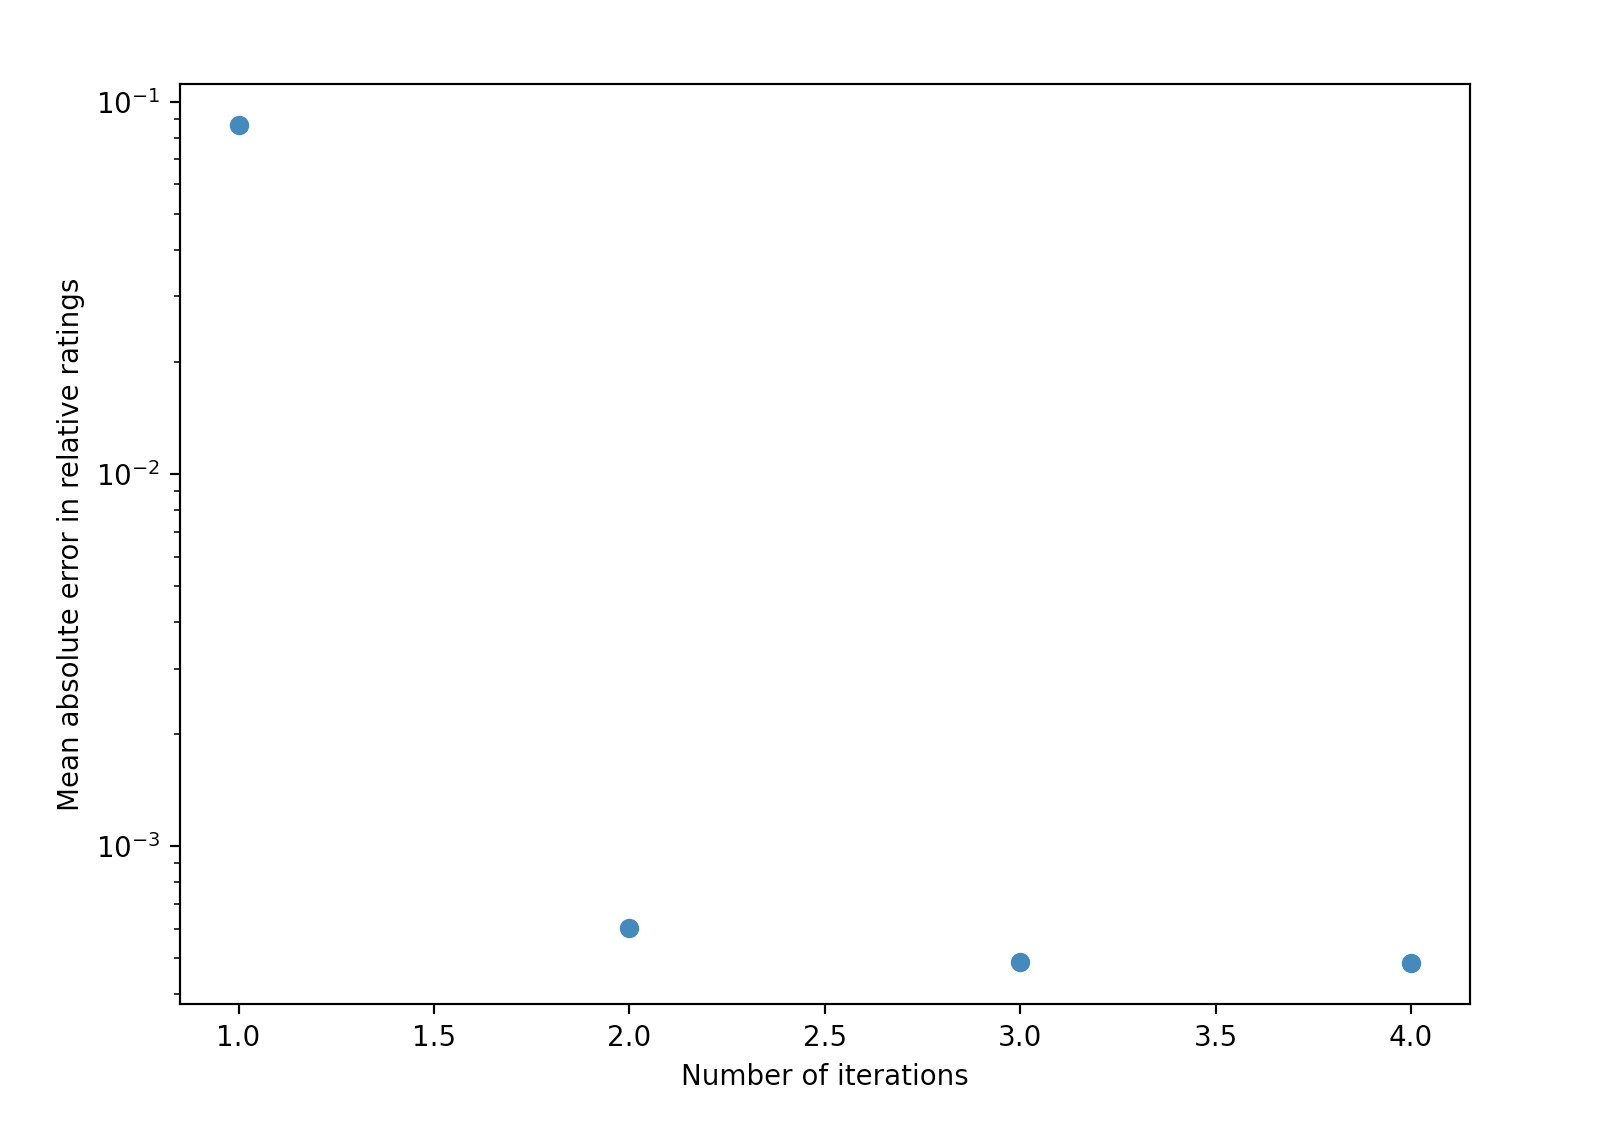
\includegraphics[scale=0.4]{convergence.png}
    \caption{Fast convergence of the iterative algorithm for relative horse ability. This example assumes a race with $100$ participants and a lattice of size $250$. A close match is achieved almost immediately. A perfect match is never achieved because the inversion algorithm is not supplied with the position of the first horse relative to the lattice, and there is a small quantization effect. This effect does not prevent close convergence to win probabilities, however - so this error will tend to overstate the numerical error that would be introduced in the pricing of quinellas or trifectas, say.}
    \label{fig:covergence}
\end{figure}

To that end, we now note that all three quantities comprising $\Upsilon$ can be quickly calculated from their equivalents without hats. Once again the easiest calculation follows from \(S_i S_{\hat{i}} = S\) where $S$ is the survival function for all horses. Thus
\begin{equation}
\label{eqn:s}
    S_{\hat{i}}(j) =  \frac{ S(j)}{ S_i(j) } 
\end{equation}
and once again, this determines the density. 
Now appealing to equation \ref{eqn:two} with the singleton horse $A=\{i\}$ and $B$ the complement, the full field multiplicity is given by 
$$
   m(j)  = \frac{m_i(j) f_i(j) S_{\hat{i}}(j) 
    + \left( m_i(j) +m_{\hat{i}}(j) \right) f_i(j) f_{\hat{i}}(j)}{f_i(j) S_{\hat{i}}(j) + f_i(j) f_{\hat{i}}(j) + f_{\hat{i}}(j) S_i(j)} 
$$
we can rearrange to determine the multiplicity with $i$ left out: 
\begin{equation}
\label{eqn:inversion}
   m_{\hat{i}}(j)  =  \frac{m(j) f_i(j) S_{\hat{i}}(j) + m(j) f_i(j) f_{\hat{i}}(j) 
     +  m(j) f_{\hat{i}}(j) S_i(j)  - m_i(j) f_i(j) S_{\hat{i}}(j) } 
     { f_{\hat{i}} ( f_i + S_i ) }
\end{equation}
This establishes a fast way to remove one horse.  

\subsection{Approximate state prices}

The final component to the algorithm is a method of estimating the state price $p_i$ under the assumption that we have been supplied with the density $f_i$ for horse $i$ and also supplied a characterization of the remainder of the horses acting as one (i.e. $\Upsilon_{\hat{i}}$ which embodies the density and multiplicity). Recall the definition of the state price. 
\begin{eqnarray*}
  p_i  & = & E \left[ \frac{ \overbrace{\iota_{ X_i=X^{(1)}}}^{horse\ i\ wins}}{\sum_k \iota_{X_k=X^{(1)}}}  \right] 
\end{eqnarray*}
We sum over all values $j$ on the lattice taken by $X_i$ and also by values $j'$ taken by $X_{\hat{i}}^{(1)}$. For brevity denote the denominator (number of ties) by 
$
      M = \sum_k \iota_{X_k=X^{(1)}}
$
the win indicator by 
$
     W = \iota_{ X_i=X^{(1)}}
$
Then splitting off the diagonal terms (ties) we have by independence of performance:
\begin{eqnarray}
\label{eqn:approximation}
p_i & = & \sum_{j,j'} f_i(j) f_{\hat{i}}(j') E\left[  \frac{W}{M} | X_i=j,X^{(1)}_{\hat{i}}=j' \right] \nonumber \\
    & = &  \sum_{j} f_i(j) f_{\hat{i}}(j) E\left[  \frac{1}{M} |X_i=X^{(1)}_{\hat{i}}=j\right]  + \sum_{j, j' > j} f_i(j) f_{\hat{i}}(j') \cdot 1 \nonumber \\
    & = & \sum_{j} f_i(j) f_{\hat{i}}(j) E\left[  \frac{1}{M} |j\right]  + \sum_{j} f_i(j) S_{\hat{i}}(j)  \nonumber \\
    & \approx & \sum_{j} f_i(j) f_{\hat{i}}(j) \frac{1}{E[M|j]}   + \sum_{j} f_i(j) S_{\hat{i}}(j)  \nonumber \\
    & = & \sum_j f_i(j) \left\{ \frac{f_{\hat{i}}}{1+m_{\hat{i}}(j)}+ S_{\hat{i}}(j) \right\}
\end{eqnarray}
The approximation in the second to last line could potentially benefit from a Jensen's Inequality estimate. However this only applies to ties and the bound $M>2$ further suggests the term arising from Jensen's Inequality is small. 
    
\subsection{Update step}
    
An iterative algorithm for determining $a_i$ from $p_i$ can now be given in Algorithm \ref{alg:inversion}. The approximate state price calculation is used to determine a lookup table from ability to win probability. Linear interpolation is use to adjust the abilities of the horses. Note that we compute \ref{eqn:s}, then $f_{\hat{i}}$ from $S_{\hat{i}}$ using the definition \ref{eqn:survival}. An example of multiplicity $m_i(j)$ is plotted for a race with three entrants in Figure \ref{fig:multiplicity}. A similar example with $25$ participants is shown in Figure \ref{fig:multiplicity25}

\begin{figure}
    \centering
    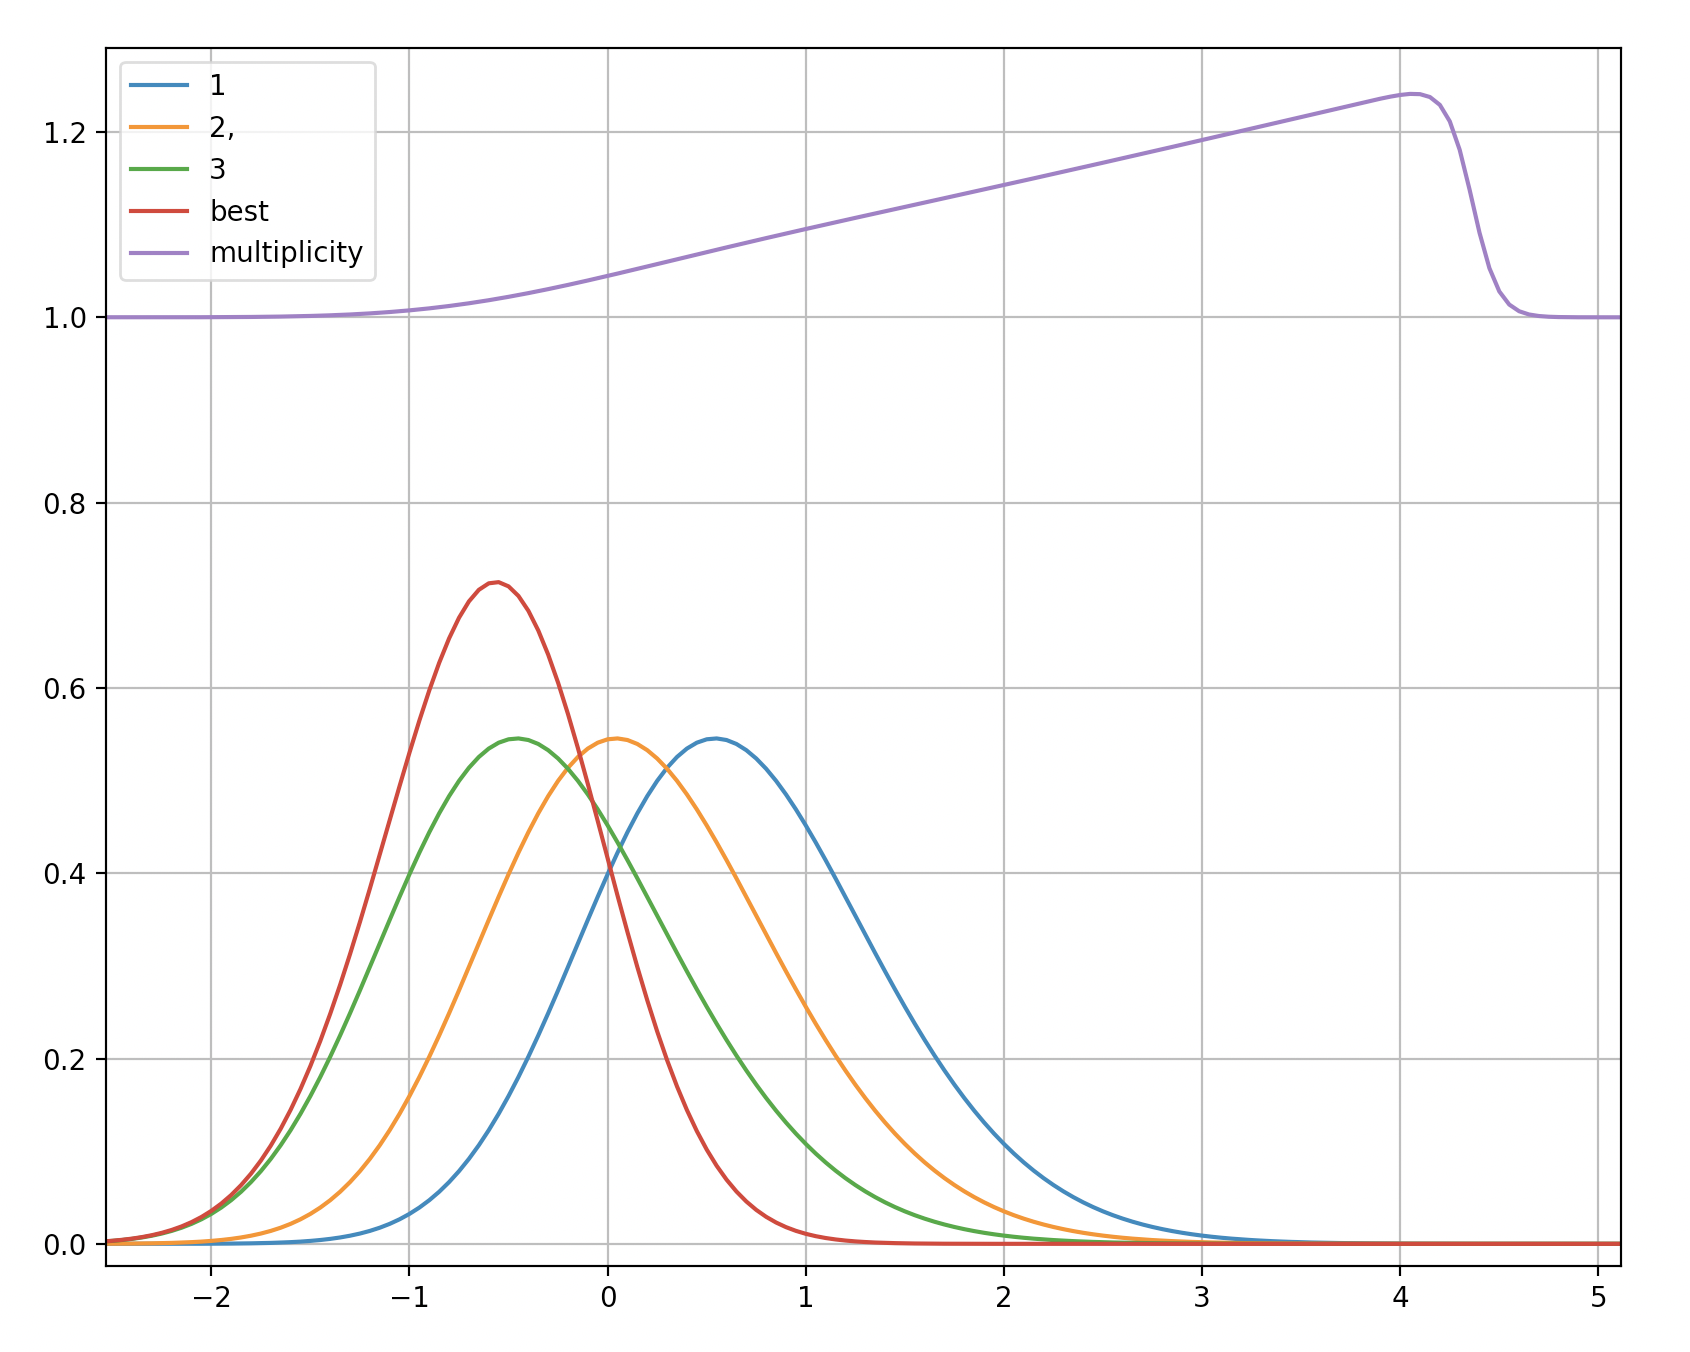
\includegraphics[scale=0.4]{multiplicity_fixed.png}
    \caption{Example of performance distributions (green, orange and blue), first order statistic (red) showing the distribution of the winning performance, and multiplicity (purple) for a race with three entrants. The red and purple curves are sufficient statistics when these three contestants are added to a race, at least as far as winning state prices $p_i$ are concerned. This example uses a lattice with $250$ points and
    skew-normal performance distributions. Note the slightly fatter right tails, and the fact that multiplicity is numerically stable well beyond the region where it matters.}
    \label{fig:multiplicity}
\end{figure}


\begin{figure}
    \centering
    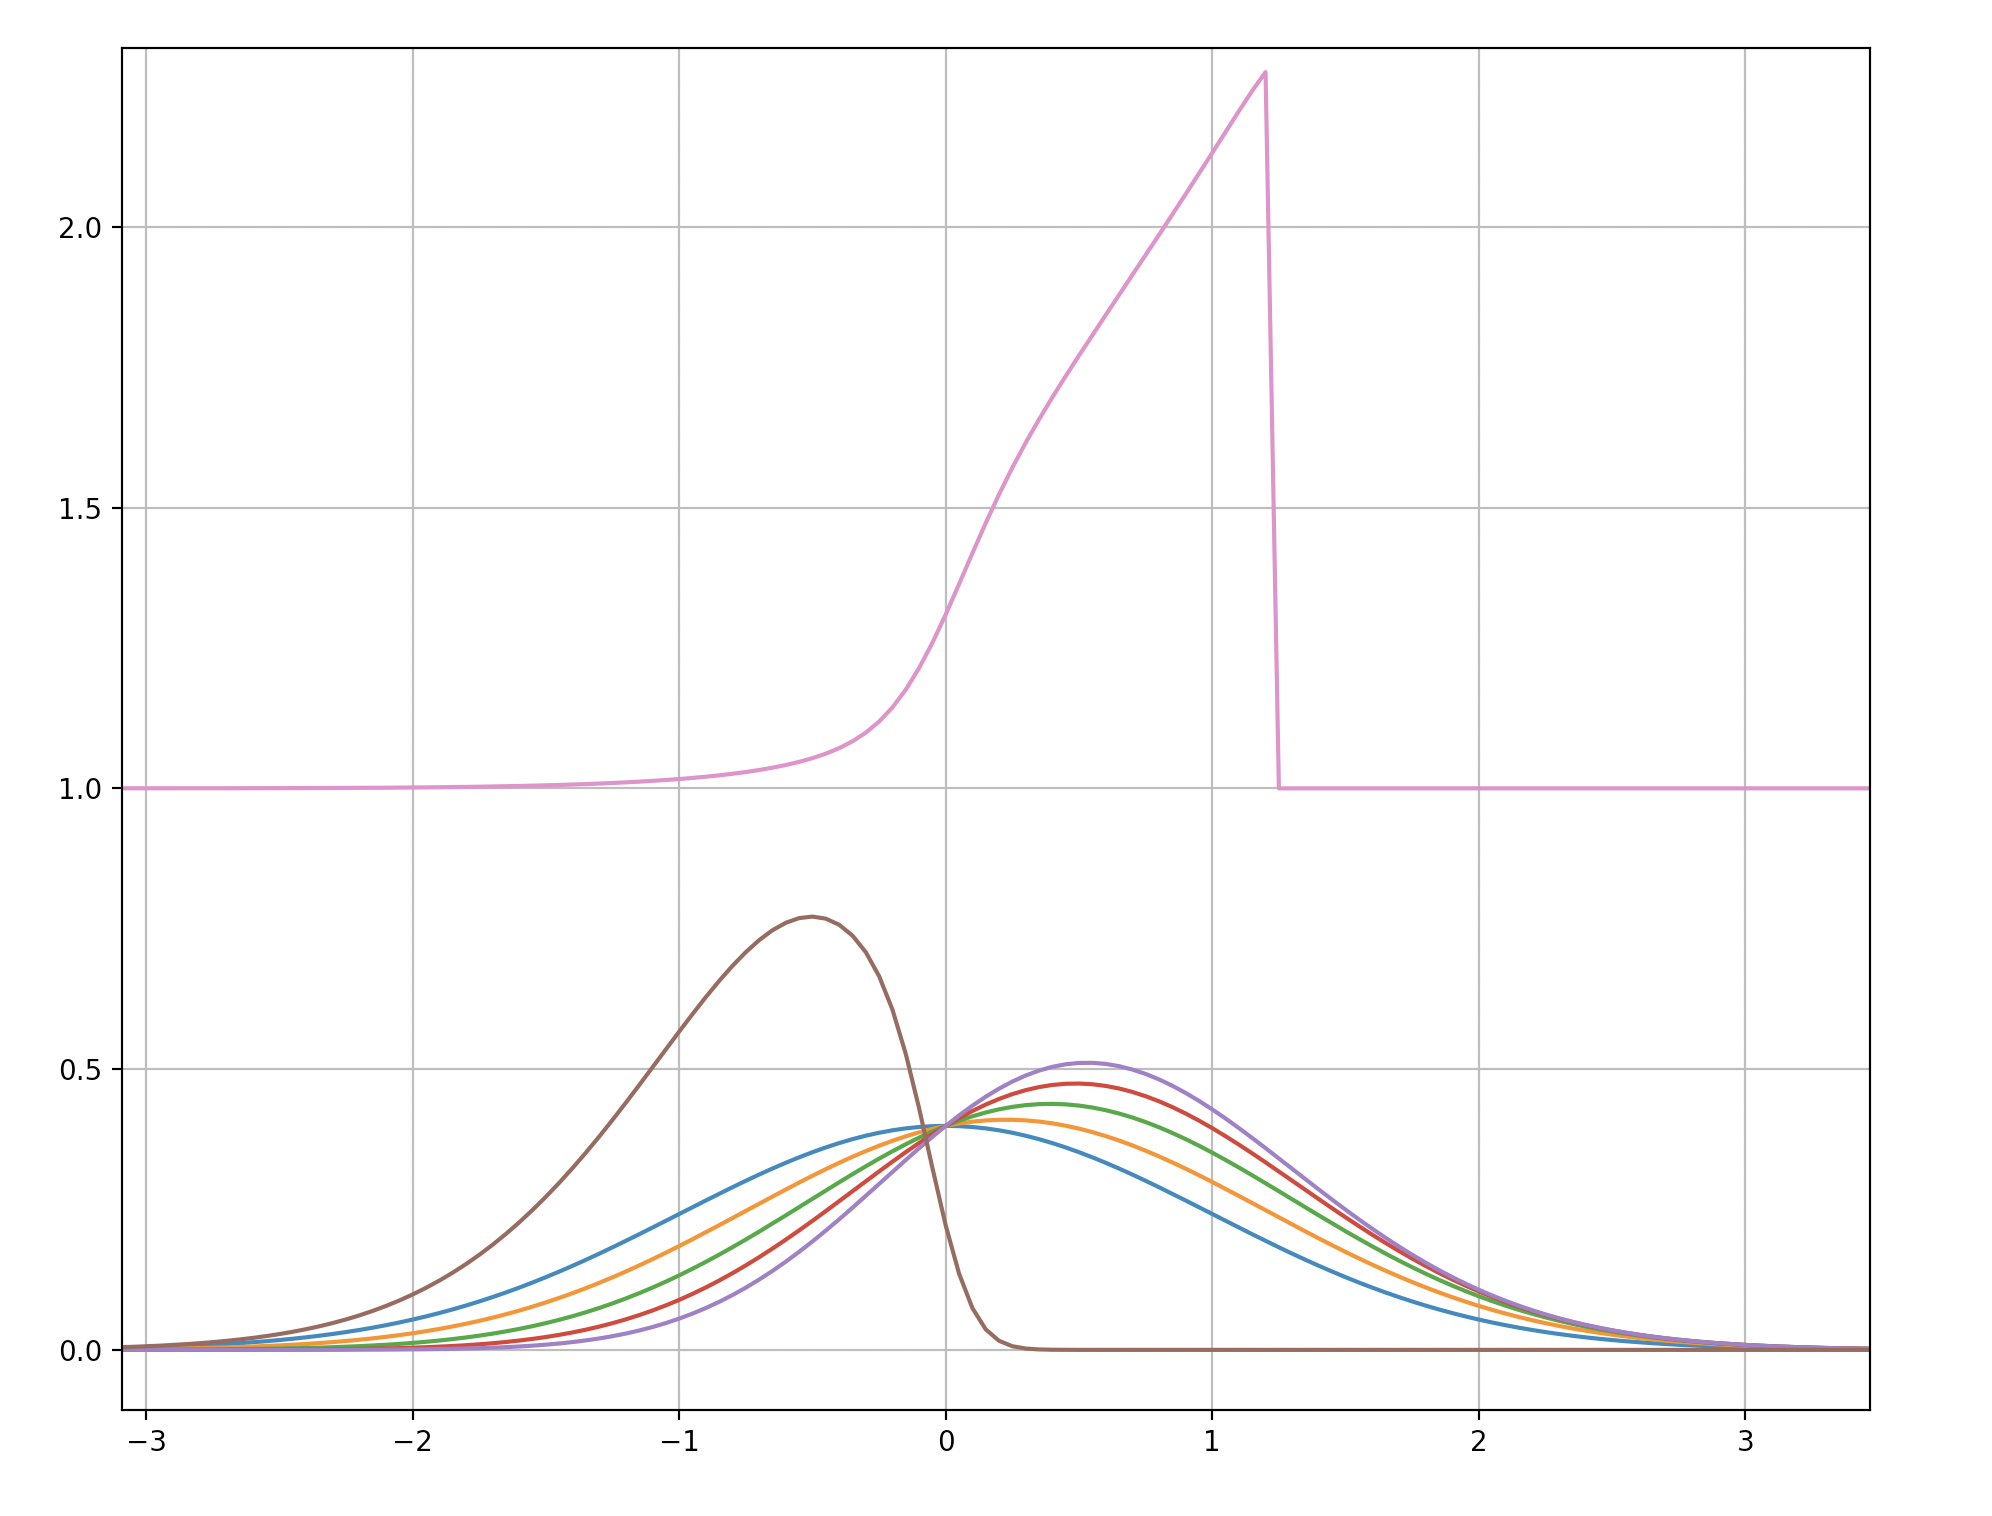
\includegraphics[scale=0.35]{multiplicities_25.png}
    \caption{Example of performance distributions, first order statistics, and multiplicity (top pink curve) for a race with twenty five entrants. Only every fifth performance curve is plotted.}
    \label{fig:multiplicity25}
\end{figure}



\begin{algorithm}[tb]
   \caption{Computing the density and multiplicity for the least of $n$ discrete random variables}
   \label{alg:multiplicity}
\begin{algorithmic}
   \STATE {\bfseries Input:} Discrete densities $f_i: \mathbb{N}\rightarrow \mathbb{R}$, multiplicities $m_i:\mathbb{N}\rightarrow \mathbb{R}$ for $i \in \{1,\dots,n\}$
    \STATE Initialize $S=S_1$ using equation \ref{eqn:survival}
    \STATE Initialize $f=f_1$, $m=m_1=1$
   \FOR{$i=2$ {\bfseries to} $n$}
   \STATE $S \rightarrow 1- (1-S)(1-S_i)$
   \STATE $f(j) = S(j)-S(j-1)$ for all $j$
   \STATE Assign $m(j)$ for all $j$ using eqn \ref{eqn:two} with $f,m,S$ taking the role of group $A$ and $f_i,m_i,S_i$ the role of group $B$. 
   \ENDFOR 
   \RETURN $m$, $S$ and $f$
\end{algorithmic}
\end{algorithm}

\begin{algorithm}[tb]
   \caption{Discrete Horse Race Calibration}
   \label{alg:inversion}
\begin{algorithmic}
   \STATE {\bfseries Input:} data $p_i$, discrete density $f$ representing common performance density up to translation. 
   \STATE Initialize $a_i=0$ for all $i$.
   \REPEAT
      \STATE Use Algorithm \ref{alg:multiplicity} to compute $S,m,f$ from densities $f_i:=f^{\rightarrow a_i}$
      \FOR{$i=1$ {\bfseries to} $n$}
      \STATE Compute $S_{\hat{i}}$, $m_{\hat{i}}$ using eqn \ref{eqn:inversion} and \ref{eqn:s}
      \STATE Compute implied state prices $\tilde{p}_i$ for all $i$ using \ref{eqn:approximation}
      \ENDFOR
    \STATE Add to the set of computed $(a,\tilde{p})$ pairs some additional implied state prices for a small number of evenly spaced, additional $a_i$ values (in order to create a stable lookup table from $a \rightarrow \tilde{p}$ used in the next step).   
    \STATE Assign new $a_i$ by piecewise linear interpolation.   
   \UNTIL $\tilde{p}_i \approx p_i$ for all $i$
   \RETURN $a_i$'s
\end{algorithmic}
\end{algorithm}

\subsection{Reference implementation}

The novelty in this algorithm lies in the use of Equation \ref{eqn:inversion} to facilitate an extremely fast iterative sweep. This obviates any kind of multidimensional parameter search. There are some other details of the reference open source implementation that bear brief comment. However their modification is not likely to make nearly as big a difference. We refer the reader to the open source code provided \cite{pysport}. There is also a calculator made available at \cite{horseapi}. 

The first comment is that given $\tilde{p}_i$'s the updating of $a_i$'s can be implemented in several ways. It was initially thought that some other monotonic transformation of $\tilde{p}_i$ would help, such as assuming log odds ratios were linear in $a_i$ (or some other approximation motivated by extreme value theory perhaps). But  surprisingly, piecewise linear interpolation leads to almost immediate convergence. The reference implementation \cite{pysport} uses numpy's interp1d linear interpolation algorithm for simplicity.

Also, it should be clear that any reasonable convergence (i.e. termination) criteria might be used, such as requiring that $\tilde{p_i}$ differ from $p_i$ by less than a fixed threshold. Of course one might assume some other criterion such as divergence of logarithms of probabilities, or of odds ratios, or standard measures of dispersion between discrete distributions.   

\subsection{Convergence}

There are two notions of convergence that might be used to test Algorithm \ref{alg:inversion}. We can start with a collection of winning probabilities, infer relative ability, recompute implied probability of winning and compare. Alternatively, we can start with relative ability and complete a similar round trip. We have already noted the second possibility and, in Figure \ref{fig:covergence}, the rapid convergence after two iterations. 

The matching of win probabilities is probably the more relevant of the two criteria, if determining pricing for exotic wagers is the intent. For $n=10$ corresponding the relative error after five iterations is on the order of 1 part in 10,000, meaning that a horse specified to have a ten percent chance of winning will have an inferred probability of winning that is within $1/100,000$ of $0.1$.  

We tested the ability to reproduce probabilities to high precision even when race size is increased. Figure \ref{fig:accuracy} reports the mean absolute relative error defined as 
$$
   relative/ error = \frac{1}{n} \sum_i \frac{|\tilde{p}_i-p_i|}{p_i}
$$
where $p_i$ and $\tilde{p}_i$ are the given and calibrated probabilities respectively. This experiment suggests that relative errors increase with the logarithm of the number of runners. However even for races of size $n=60,000$ this corresponds to a relative errors on the order of five one hundredths of a percent. 

\begin{figure}
    \centering
    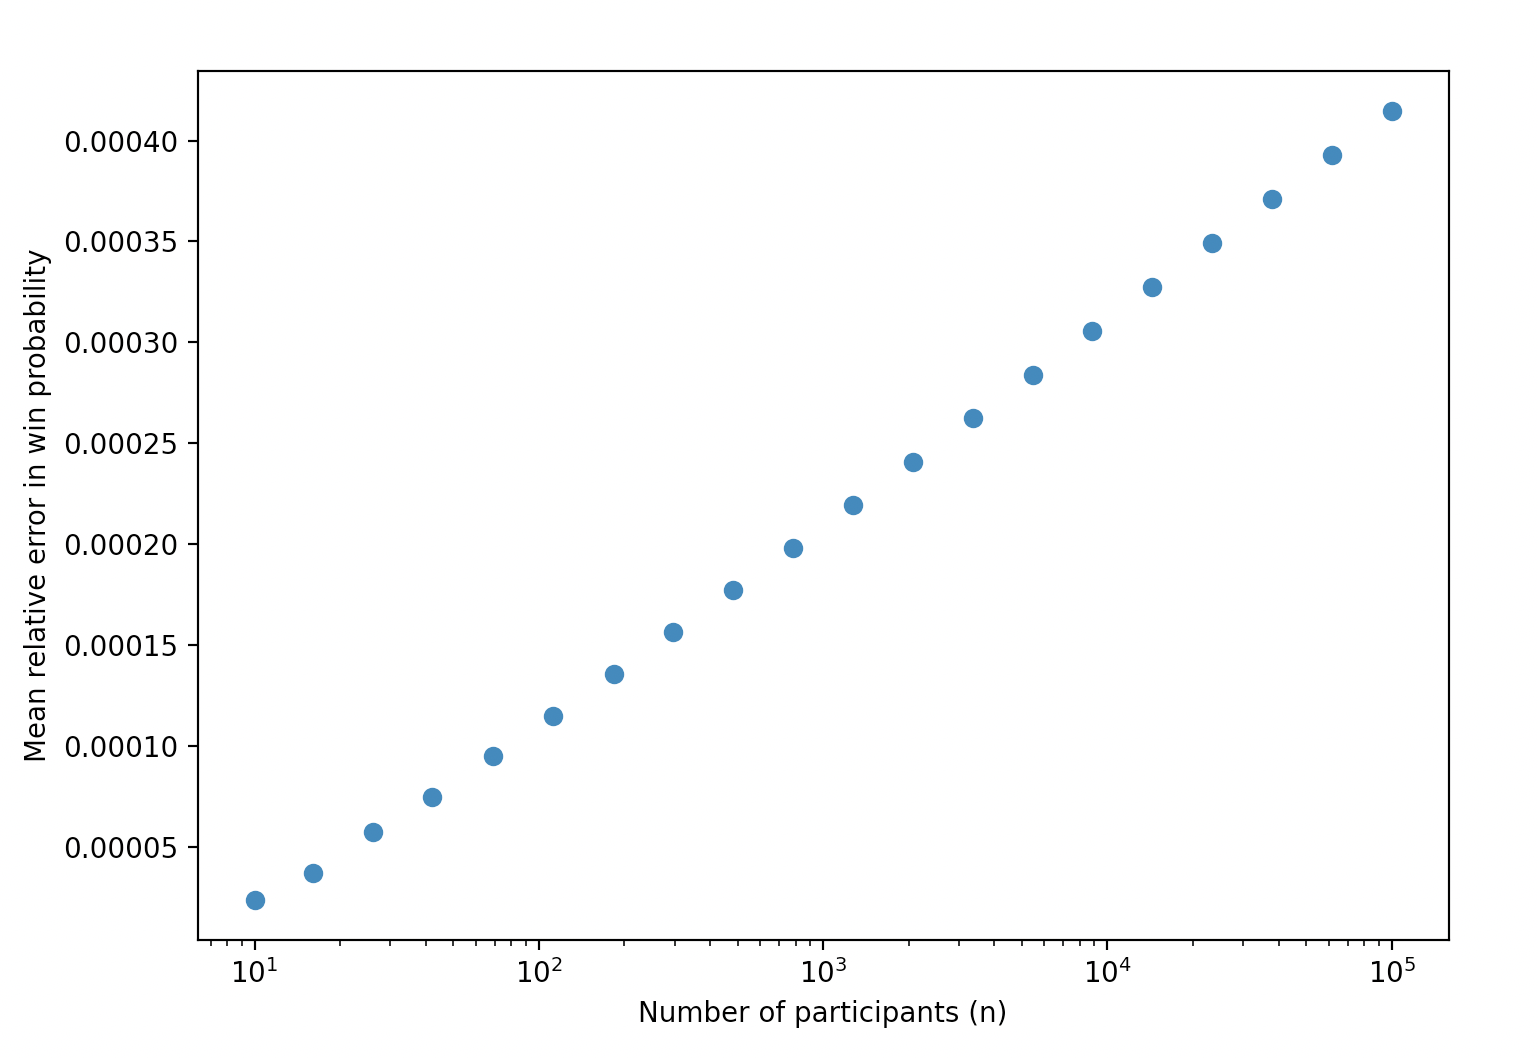
\includegraphics[scale=0.4]{accuracy.png}
    \caption{Relative error in calibrated versus supplied probability as a function of race size $n$. Even for a race with $60,000$ entrants, the relative error between supplied and calibrated win probability is on the order of hundredths of a percentage point.}
    \label{fig:accuracy}
\end{figure}

We do not provide a proof of convergence, which is an acknowledged shortcoming at present. The definition we have used for translation in the formulation of the discrete horse race problem guarantees monotonicity in winning probability as we vary $a_i$. Thus, in establishing that an $a_i$ can be chosen to match $p_i$ holding all other $a_j$ constant (and absent non-degenerate cases such as the one mentioned above) the intermediate value theorem suffices. This suggests, but does not prove, convergence of the vector $\tilde{p}_i$ to $p_i$ using the accelerated algorithm we suggest (in which all $a_i$'s are altered simultaneously).

It is worth noting that this algorithm, or any other, cannot converge for degenerate choices of $f^*$ if no solution exists! For instance if $f^*$ takes only one value, it will evidently be impossible to calibrate a translation family matching any set of winning probabilities other than $(1,0,\dots, 0)$, $(\frac{1}{2},\frac{1}{2},0,\dots, 0)$ and so on. 


\subsection{Computational performance}

\begin{figure}
    \centering
    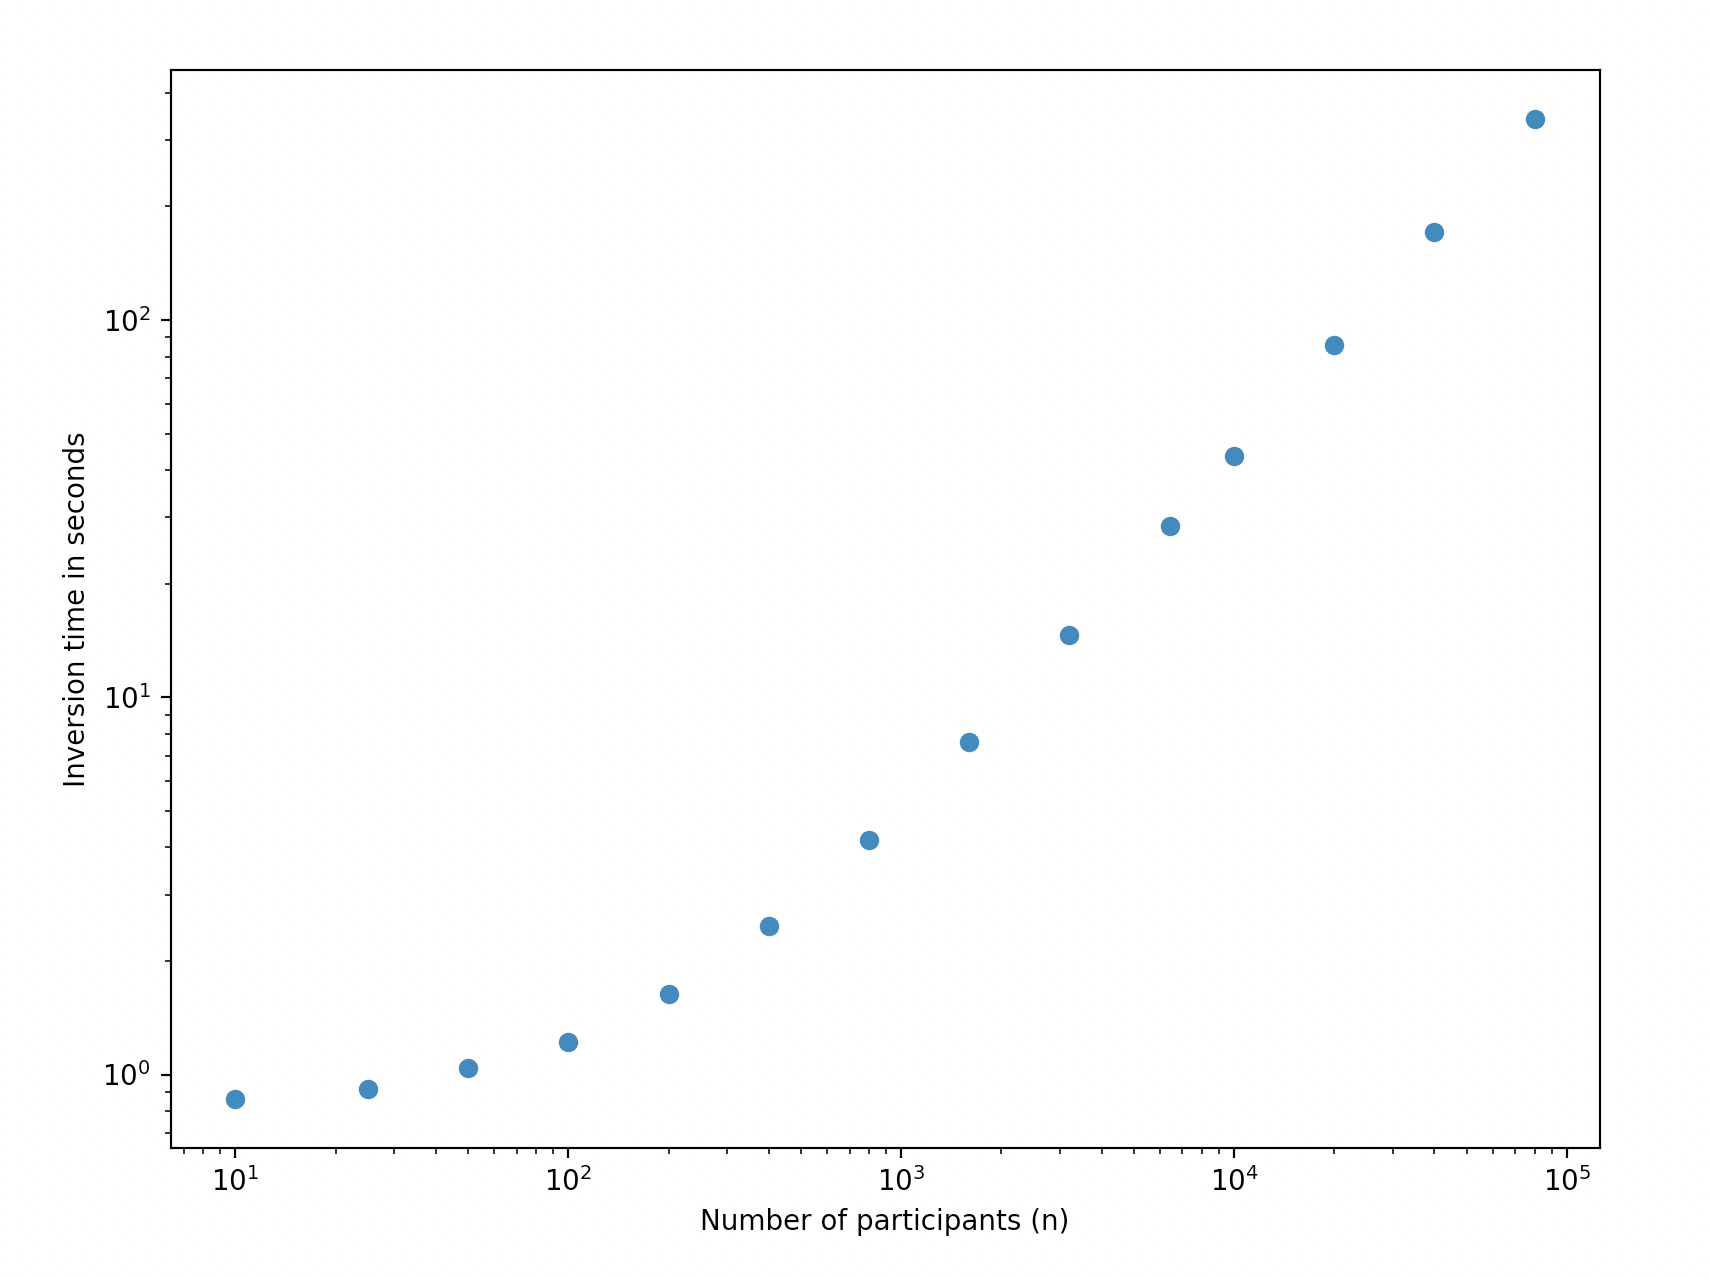
\includegraphics[scale=0.4]{performance.png}
    \caption{Computation time of the Python reference implementation of Algorithm \ref{alg:inversion}. Five iterations were used, and a lattice size of $500$. Running time is initially super-linear due to one part of the algorithm being relatively inefficiently implemented in Python. But for large $n$ running time is empirically sub-linear. Ability can be implied for a race with $n=1000$ horses in a few seconds, or $n=100,000$ if one has more time (despite the fact that the latter is ostensibly a $99,999$ dimensional optimization.)}
    \label{fig:one_thousand}
\end{figure}

We claim this algorithm is fast. For races up to size $n=1000$ the calibration using Algorithm \ref{alg:inversion} is accomplished in a few seconds, as illustrated in Figure \ref{fig:one_thousand}. As the obvious alternative would involve fitting a model with $999$ free parameters and thus a $999$ dimensional optimization, it is unclear how this should best be benchmarked.  

A further difficulty in finding comparable algorithms arises from the scaling performance of Algorithm \ref{alg:inversion} well beyond $n=100$ or $n=1000$, which are typical upper limits of the dimensionality of problems for which most optimization routines are intended. In contrast Algorithm \ref{alg:inversion} is more akin to a fast inversion of a band matrix, or some other equally fast and scalable technique taking advantage of a special setup.  
As demonstrated in Figure \ref{fig:one_thousand} the growth in computation time is approximately linear as $n$ rises (empirically slightly sub-linear, in fact). This is to be expected for Algorithm \ref{alg:inversion} given the efficiency of one dimensional linear interpolation in numpy, and the fact that Algorithm \ref{alg:multiplicity} is called only once per cycle. 

Clearly the specific nature of the horse race problem or the pattern of the $a_i$ must be incorporated in some way, if we are to create any kind of benchmark to \ref{alg:inversion} that has remotely comparable performance. Any alternative technique that calls into a multi-dimensional optimization routine at some point will surely fail to match the match the linear performance of Algorithm \ref{alg:inversion}.\footnote{Potentially, swarm optimization or other techniques designed for very high dimensional problems might be used, but are likely to be slower by many, many orders of magnitude by the time we get to $n=1000$, never mind $n=100,000$.  
} For this reason we do not know what a reasonable alternative might be, or, dare we say, how to arrange an interesting horse race between horse race calibration algorithms.  

As noted, we previously attempted to use a low dimensional parametrization of the $a_i$ together with general purpose solvers in \cite{cotton_blog}, and this did lead to order of magnitude improvements - though still nothing remotely comparable to Algorithm \ref{alg:inversion}. A further drawback with this prior work is that it did not lead to tight calibration of the probabilities. 

\section{Implications}
\label{sec:implications}

In this section we establish that some models made practical by Algorithm \ref{alg:inversion} will differ markedly from prior approaches when it comes to assigning probabilities, and therefore the space of models opened up is important. However we also explain why that is not the only implication. The use of explicit performance models (parametrized by a performance distribution $f^*$ and relative abilities) is not widespread but is likely to become so as in-the-run wagering grows in popularity. 

There are other ways in which a fast algorithm for solving for $a_i$'s when $p_i's$ and $f^*$ are known can further research, and there seems to be no difficulty presented. For example, any choice of $f^*$ will imply a likelihood on race outcomes and thereby, different choices of $f^*$ will lead to more or less accurate empirical performance over time.   

\subsection{Deviation from axiom of choice in exacta pricing}

We first demonstrate that the choice of $f^*$ greatly influences probabilities of joint outcomes - such as the probability of two particular horses finishing first and second in a given order. It follows from this that it is dangerous to assume exponential running times, or equivalently assume Luce's axiom of choice holds, even if runners are assumed to be independent.   

Starting with a three horse race where winning probabilities are $p_1=1/2$, $p_2=1/3$ and $p_3=1/6$ we compute the extent to which the conditional probability of finishing second deviates from the axiom of choice. Table \ref{tab:exacta} reports the percentage differences in probability for each of the six possible outcomes. The increase in likelihood can be as much as thirty percent. 

\begin{table}[]
    \centering
    \begin{tabular}{|c|c|c|c|}
    \hline 
    & $p_2=1/2$ & $1/3$ & $1/6$ \\
    \hline 
$p_1=1/2$ &    & -8.10 & 16.3 \\
$p_2=1/3$ & -10.2 & & 30.5 \\
$p_3=1/6$ & -5.70 & 8.50 & \\
\hline
    \end{tabular}
    \caption{Percentage increase in exacta probability relative to Harville's formula for a three horse race with winning probabilities $1/2$, $1/3$ and $1/6$, assuming normally distributed performance. For example the chance of the lest-favored horse finishing second behind the second-favored horse is thirty percent higher in this model than the axiom of choice (Harville model) would suggest. Harville predicts a probability of $\frac{1/3 \times 1/6}{1-1/3} = 1/27$ for this ``exacta'' outcome. Normal independent performance suggests a probability closer to $1/19$.}
    \label{tab:exacta}
\end{table}

We also repeated that experiment for a larger field (using odds for the 2020 Kentucky Derby as a guide). In the interest of space we do not report the exacta matrix, but we found even bigger discrepancies. Exacta probabilities involving horses with odds over $100/1$ differed by a factor of $2$ compared to their Harville equivalents. This effect was even more pronounced when normally distributed performance was replaced by skew-normal. 

\subsection{Scratchings}
\label{sec:scratching}

When a horse is removed from a race at a late stage, it is the custom to refund wagers. However this is unfair to bookmakers who have offered fixed prices on the other horses, whose winning probabilities have now improved. The customary remedy is an after the fact reduction in payments (i.e. odds). This reduction is based on Luce's axiom of choice, which is to say a simple rescaling. We would submit that a more equitable approach would involve a computation of reductions using some plausible choice of $f^*$, and Algorithm \ref{alg:inversion}. 

\subsection{Deviation from the bookmakers' quarter rule for show wagers}
\label{sec:quarter}

A longstanding practice amongst bookmakers sets the odds for a show bet at one quarter of the odds for a win bet. A show wager, in this note, refers to a bet that a horse will finish first, second or third.\footnote{We use U.S. terminology where place refers to top two and show to top three. In Australia place refers to top three in fields with eight or more runners.} The quarter rule is not always offered for show betting in isolation, but for a combination of a win and a show bet (called an each-way bet). The return on longer priced horses is typically poorer than for shorter priced, so the rule of a quarter can sometimes be viewed as an enticement to enter an each-way bet. Setting aside these issues and the bookmaker's typical profit (greater for less favored horses), the quarter rule implies the following ratio between show and win probability: 
$$
    \frac{P(win)}{P(show)} = \frac{ p }{ 4/(p+1) + 1 }
$$
where $p=1/(o+1)$ is the probability implied by bookmaker odds quoted as $o:1$. For example, an even money favourite with $o=1$ is assigned odds of $1/4$ of finishing in the top three (meaning an eighty percent chance). We compared this heuristic against show probabilities implied by skew-normal performance distributions. 

Once again using probabilities inspired by the Kentucky Derby long range odds, Table \ref{tab:show} reports the normalized bookmaker odds, quarter rule show odds, quarter rule show probabilities and skew-normal model show probabilities for all runners. As is readily apparent (and not altogether surprising) the presence of a pronounced favourite makes it perilous for bookmakers to apply the quarter rule. The probability of less favored runners finishing in the top three is substantially higher that the rule of a quarter would suggest. 

\begin{table}[]
    \centering
    \begin{tabular}{|c|c|c|c|c|c|}
    \hline 
        &  Bookmaker & Bookmaker & Bookmaker & Skew model & \\
    Rank &  Win & Show & P(show) & P(show) & Difference (\%)  \\
    \hline
0 & 1.382&0.345&0.743&0.651&-12.4 \\
1 & 8.423 & 2.106 & 0.322 & 0.311 & -3.5 \\
2 & 10.442 & 2.61 & 0.277 & 0.271 & -2.2 \\
3 & 13.807 & 3.452 & 0.225 & 0.23 & 2.2 \\
4 & 27.268 & 6.817 & 0.128 & 0.144 & 12.6 \\
5 & 27.268 & 6.817 & 0.128 & 0.144 & 12.4 \\
6 & 33.998 & 8.5 & 0.105 & 0.124 & 18.0 \\
7 & 38.037 & 9.509 & 0.095 & 0.113 & 18.7 \\
8 & 40.729 & 10.182 & 0.089 & 0.109 & 22.0 \\
9 & 44.767 & 11.192 & 0.082 & 0.1 & 22.5 \\
10 & 54.19 & 13.547 & 0.069 & 0.087 & 26.9 \\
11 & 54.19 & 13.547 & 0.069 & 0.088 & 28.3 \\
12 & 67.651 & 16.913 & 0.056 & 0.073 & 31.6 \\
13 & 74.381 & 18.595 & 0.051 & 0.069 & 34.7 \\
14 & 89.188 & 22.297 & 0.043 & 0.059 & 36.6 \\
15 & 89.188 & 22.297 & 0.043 & 0.059 & 38.4 \\
16 & 108.033 & 27.008 & 0.036 & 0.051 & 43.8 \\
17 & 108.033 & 27.008 & 0.036 & 0.052 & 44.4\\
18 & 134.955 & 33.739 & 0.029 & 0.043 & 49.5\\
19 & 134.955 & 33.739 & 0.029 & 0.043 & 49.8\\
20 & 134.955 & 33.739 & 0.029 & 0.043 & 49.4\\
21 & 168.608 & 42.152 & 0.023 & 0.036 & 56.1\\
22 & 168.608 & 42.152 & 0.023 & 0.036 & 53.5\\
23 & 202.26 & 50.565 & 0.019 & 0.032 & 63.6 \\
24 & 202.26 & 50.565 & 0.019 & 0.032 & 64.5 \\
\hline 
    \end{tabular}
    \caption{Comparison between the bookmaking rule of a quarter show probability (finish in the top three) computed using skew-normal performance distributions. We use ordered, normalized early bookmaker odds for the Kentucky Derby (as of August 22, 2020). The bookmaker convention applied to the favorite implies that a bookmaker risks $1.382$ for every dollar a patron risks when that take a win bet, whereas for a show bet the bookmaker risks $0.345$ to the patron's dollar (one quarter). Break even probabilities are shown for show betting. The skew-normal performance model is calibrated to the bookmaker implied probabilities (not shown) using Algorithm \ref{alg:inversion}. The data suggests that less favored horses have a much higher chance of finishing in the top three than the quarter rule would suggest. However this discrepancy might be reduced or eliminated entirely were we to perform a power transform on horse probabilities prior to normalization, or otherwise account for lower returns on longer priced horses (known as the longshot effect). Moreover, show bets are often only available when bundled with win bets. For these reasons this table does not necessarily suggest positive returns are available, despite the large discrepancy. In generating this table a parameter $\alpha=2.0$ for the skew-normal distribution was used.}
    \label{tab:show}
\end{table}

\subsection{A pricing measure for all wagers determined by finish positions}

Because the distribution of the individual $X_i$ is not assumed but left general, the user of Algorithm \ref{alg:inversion} is granted great flexibility. In particular, varying $f^*$ generates different families of pricing schemes for quinellas, trifectas and other types of exotic wagers - all of which are consistent with observed win prices. Some of those pricing methodologies may be more accurate than others, possibly much more accurate than Harville. 

Indeed, if we recklessly make the assumption that the win market for horse racing contains most of the information (and quinellas, exactas and all other varieties of combinatorial bets are mere derivatives of the win market) then Algorithm \ref{alg:inversion} defines a coherent and in some sense comprehensive solution for the pricing of all possible claims which are contingent on the realized rank order of finishers.  

We hastily add, in the interest of the reader's financial well-being, that there is strong reason to believe not all information is absorbed into win prices. One reason is that professional handicappers achieve more leverage in combinatorial markets, and thus trifecta markets can provide additional information (and might even be more efficient than win markets). That is why we have suggested that varying $f^*$ in order to calibrate to additional market information might be a worthwhile improvement. 

\subsection{... and some that are not.}

Furthermore, with further calibration of the scale of $f^*$ (leaving probabilities for rank determined events unchanged) it will be possible to price derivatives which settle on outcomes other than finishing position. For example, with an empirically estimated scale parameter it is possible to price wagers that settle based on the relative finishing times of two horses. These are known as spread bets. 

\subsection{Feature generation}

The reader intent on tackling the horse racing markets might wish to view this contribution as a technique for generating features $a_i$ from market prices $p_i$. Those features can then be used in conjunction with additional data to predict more accurate estimates. For instance the $p_i$ might enter an empirical iterative, probit or logistic regression model as in  \cite{compleat}, \cite{Lo2006ACompetitions}, \cite{Bolton2008SearchingRaces},  conveyed verbally in \cite{probit_talk} and anecdotally used widely by successful handicapping syndicates. 

Using transforms of market probabilities as predictive features is also considered for soccer forecasting \cite{Wunderlich2018TheSoccer}. As a more general comment it is well appreciated that mapping probabilities $p_i$ onto quantities that are closer to being normally distributed can allow the researcher to exploit a wider range of methods such as Kalman filtering or gaussian processes. Beyond wagering this may also assist the econometric literature that uses racetracks as laboratories \cite{Camerer2002CanBetting} to draw wider conclusions about asset markets, or as a lens into human behaviour such as risk preference and perceptions of probability \cite{ErikSnowberg2010ExplainingMisperceptions}, \cite{Williams2003WhyMarkets} \cite{Thaler2012Anomalies:Lotteries}, \cite{Asch2002MarketCorrection}. 
\subsection{Ratings and implied observations}

Chess players have long been rated using the Elo system - which is roughly consistent with normal $f^*$ or logistic $F^*$ depending on the implementation. Normally distributed performance and Bayesian updating on a graph has been used in improvements to the Elo system \cite{2018TrueSkill:System}. Typically these rating systems use updates based on actual realized results. However there is no reason why market information cannot also be incorporated. When implied abilities $\{a_i\}_{i=1}^n$ are interpreted as a result, they too can be fed into any rating system. The importance of price implied updating versus result implied updating can be estimated from empirical data. 

\subsection{Pre-post price fluctuations}

Another practical application of the transform $\{p_i\} \mapsto \{a_i\}$, that we have established in Algorithm \ref{alg:inversion}, is the modeling of the time varying dynamics of prices in a multi-entry contest {\em prior} to the event. Pre-event bookmaker and parimutuel price fluctuations are studied intently by professional handicappers and our approach provides them with a different, and perhaps more convenient, parameterization of prices. For instance $f^*$ may be chosen to be normal, lognormal or some other convenient distribution admitting a correspondingly convenient stochastic process on the $a_i$. This in turn confers a stochastic process on $p_i$. 

\subsection{In-the-run wagering}
\label{sec:intherun}

While relative ability might be a convenient way to consider pre-event price fluctuations, the use of Algorithm \ref{alg:inversion} or an alternative is even more strongly motivated, dare we say mandatory, if one is required to model price changes after the event has begun. The reader will not that relative ability is arbitrary up to a scaling factor, since the performance distribution $f^*$ can be scaled. By choosing this scaling carefully, $f^*$ may be chosen to relate directly to measurable progress in a contest (such as score to par in a golf tournament) and, thereby, price estimates or probabilities may be updated.  

\subsection{Possible extensions}

As a technical comment, we assumed in our description of the algorithm that each variable took on the same distribution $f^*$ up to translation. The careful reader will observe that this is leveraged only in the interpolation step, and that with care it may be possible to generalize. For example a large number of horses may take on a small number of choices of $f^*$'s. 

A further limitation is that horse performances has been assumed to be independent. This may not prevent the approach from improving on Harville, where horses are also independent, but one can certainly question the generality of this assumption. For example in the ``straight six'' race held at Flemington Racecourse the field will sometimes bifurcate into two packs, one running the inside rail and one the outer. Differing track conditions will induce strong dependency. Another source of dependency is preference for pace. 

It may be possible to generalize Algorithm \ref{alg:inversion} to allow for probabilities that are influenced by a single common factor (such as race pace) - for instance by the use of a Normal Copula with constant off-diagonal correlation matrix applied to win probabilities. This will, however, be more computationally expensive. 

\section{Commercial Uses}
\label{sec:applications}

We now leave behind wagering - though the title of this section is not intended to suggest that horseracing markets are not economically significant in their own right (on the contrary, it is not unusual for hundreds of millions of dollars to be bet on a single race meeting).\footnote{In Hong Kong, Sha Tin and Happy Valley racecourse regularly report meeting volumes between \$$100$m and \$$200$m USD. The Melbourne Cup volume is estimated at \$$350$m AUD.} However, horseracing volumes pale in comparison with equity block orders, over the counter financial markets and the sum over all categories of trading activity in art, materials, apartments and illiquid goods of all varieties. We shall demonstrate an application of Algorithm \ref{alg:inversion} to trade of most kinds.  

Algorithm \ref{alg:inversion} is also a basic tool for the study of order statistics and rankings. It will find many applications far from the racetrack any time empirical evidence for ``ability'', broadly defined, manifests as probability that one item out of several presented is chosen. 

\subsection{Trading and the cost of inquiry}
\label{sec:trade}

A fundamental decision when selling an asset, and in some stylized setups the only decision, is the set of people to reach out to. When a party seeks to buy or sell a large amount of a stock, or a corporate bond, or a used car, they will often seek price quotes from several dealers. We present an approach to dealing with this ubiquitous problem of trade in which Algorithm \ref{alg:multiplicity} is used once, and subsequently Algorithm \ref{alg:inversion} is used repeatedly. 

In this stylized version of trade each dealer is participating in a sealed bid auction and the customer will take the best price offered. This pattern of behaviour has not been replaced by electronification, except for a few cases where central limit order books prevail. Electronic venues for government and corporate bond trading continue to use variations of a ``request for quote'' (RFQ) protocol. In essence, this replaces a phone call with an electronic message to a chosen set of dealers, but does not otherwise alter the nature of trade, or the core decision: who to contact.\footnote{Examples include TradeWeb and MarketAxess}.

For most assets there are material economic costs of inquiry. For smaller assets the direct expense as a proportion of the asset's worth can quickly mount up, especially if inquiry is time consuming (as with filling out lengthy forms at a car dealership). For larger assets the more important cost is information revelation.  

An inquiry might be construed as information about portfolio holdings or future trading intent. A call to an art dealer about a treasured family hierloom might be construed as personal financial distress, modifying the behaviour of the dealer the next time an inquiry is made and perhaps the behaviour of any other dealer catching wind. Thus all else being equal the holder of an illiquid security might prefer to indicate the desire to trade in that security only to a small number of market participants. 

The tradeoff between inquiry cost and expected price improvement is usually left to judgement - but there is no reason why a calculation cannot assist or even replace a human in the task of choosing a subset of people to reach out to. To formalize we will assume the inquiry cost is a parameter set by the customer, presumably informed by their opinion as to the likely behaviour of the counterparty. On the other hand, we directly model the best price distribution as a function of who is called. 

To this latter task, we note that {\em in theory} a customer might, with sufficient information, construct a detailed model for the joint distribution of dealer responses - and then by further optimization determine the best subset of dealers to call. In practice this will be unwieldy for the majority of market participants. Instead we provide, using Algorithm \ref{alg:inversion}, a relatively simple parameterization of the problem which requires the customer to enter only one number for each dealer. That number is (as the reader would anticipate) the probability $p_i$ that the dealer will return with the best price.

Adopting terminology from \cite{cotton_papanicolaou} (where the same setup is considered from the dealer's perspective) we assume $n$ dealers are aware of a true value of an asset $\pi$ and, when asked to bid on this asset respond with a bid of $\pi-m_i(\omega)$ where $m_i$ is the markdown of the $i$'th dealer.\footnote{For clarity we speak only of the case of selling an asset. In the case of buying the cost is the markup rather than the markdown. Equation \ref{eqn:utility} still applies.} Our notation emphasizes that $m_i(\omega)$ is a random variable with $\omega \in \Omega$, some probability space. We assume the markup for the $i$'th dealer has translated density $f^{*\rightarrow a_i}()$ for some parameter $a_i$. 

The owner of the asset must decide who to call by minimizing the aggregate cost (markup over the fair price, plus the search cost). We write this 
\begin{equation}
\label{eqn:utility}
   V^* = argmin_{V \subset S} \left\{ x E\left[ \min_{i \in V} m_i \right] + I(V;x) \right\}
\end{equation}
where $x$ is the size of the potential trade, $S = {1,\dots, n}$ is the set of all dealers, $V$ is a subset and $I(V;x)$ is the economic cost of revealing the information to all dealers in this set. Again, $I(V;x)$ is exogenous whereas the expected markdown for the best response is to be estimated based on limited information about the dealers. 

We assume that if all dealers are asked then the unconditional probability of the $i$'th dealer providing the best price is $p_i$. The quantity $p_i$ may be informed by market share statistics if more relevant idiosyncratic statistics are not tracked by the customer. Market share numbers are often publicized or can be indirectly inferred.  
The quantity 
\begin{equation}
\label{eqn:phi}
\phi(V) = E\left[\min_{i \in V} m_i \right]
\end{equation}
can be computed by first calibrating $f_i$, the density of markdown choice, to the collection $p_i$ of market share statistics using Algorithm \ref{alg:inversion}. In the appendix, we provide a proof that this set optimization problem that results is a sub-modular minimization and thus, informally speaking, easy.

We remark that Algorithm \ref{alg:inversion} may be particularly useful because it leaves open the specification of $f^*$ and therefore can accommodate quantized, skewed, or fat tailed markup distributions. In some markets convention dictates that disseminated prices lie on a discrete lattice. Skewed markups can also be a requirement because missing a trade is a small loss compared to taking on a losing trade (the problem of adverse selection rarely escapes the mind of a cautious dealer, so modeling one sided bids or offers with a skewed distribution is natural).

\subsection{Search, recommendation and placement}

In web search a horse race occurs every time a search phrase is entered. The winner of the race is the link that is clicked on. Risk neutral win probability ($\{p_i\}$) may not exist in quite the same fashion at the racetrack, but the vast number of searches that occur (at least for common phrases) leads to a precisely defined set of $\{p_i\}$ nonetheless. 

The position of a link on the page strongly influences the user's decision (not completely dissimilar to horseracing where barrier position also matters) but we shall assume we are in the experimental phase and that a random permutation is applied so as not to bias any particular link. The user might in theory scroll or page down many times, so the size of this particular horse race might well run into the hundreds or more. 

An analogous situation occurs in e-commerce, where there may be sufficient volume to accurately imply a probability that a product wins out over others in a given category. Similarly, there are services that try to estimate which image of a house or clothing item a person might click, when presented with numerous possibilities arrayed randomly. These are examples of contests occurring with high velocity. The problem is not the estimation of $\{p_i\}$'s from a surfeit of historical data, but rather, inferring what probabilities will apply when a new very similar search is performed, or when some results are removed (in analogy to the scratching of a horse from a race, as considered in Section \ref{sec:scratching}). 

Let us further suppose that at some cost, which might be direct or indirect, it is possible for an owner of a business to improve the underlying ``ability'' of their link to attract a click. This ability is related to numerous characteristics, depending on the venue, but examples might include an investment in search engine optimization, effort put into content creation, brand awareness or other activity intended to increasing the likelihood of selection (it may even be possible to directly estimate the influence of factors such as relevance, logarithm of site popularity and so on, even if the underlying mechanics of search are opaque). 

In this setting a shift in ability to attract click-throughs, purchases or whatever constitutes a business outcome (a call to a real estate broker, for example) will come at a cost for business $i$, but the benefit will be proportional to the change in $p_i$. This is directly analogous to an updating of probabilities after a sporting event has started, as considered in Section \ref{sec:intherun}, and therefore the application of horse race calibration algorithm \ref{alg:inversion} is clear. To tie this back to the example of trade considered in Section \ref{sec:trade}, we note that a dealer responding to inquiry may also benefit from exactly the same calculus. 

\section{Summary}

We have provided a fast and scalable algorithm \ref{alg:inversion} for inferring the relative location of univariate variables $\{X_i\}_{i=1}^n$ sharing a common distribution up to translation. The evidence used is the probability of variable $i$ taking the lowest value. We approach this formally via the discrete horse race problem where distributions are supported on a set of evenly spaced points, ties are permitted, and the constraints provided are not probabilities but closely related state prices defined by formula \ref{eqn:state}. 

This algorithm is likely to be particularly useful when information informing ability relates predominantly to winning probability, and: 
\begin{enumerate}
    \item It is necessary to infer winning probabilities for a subset; or 
    \item It is necessary to infer probabilities on events defined by more than one variable (such as the probability that
    $X_i$ takes the least value and $X_j$ the second least); or  
    \item Ability finds interpretation as an expected scoring differential, and it is necessary to 
    infer probabilities after scores have been updated.
\end{enumerate}
For this reason the algorithm finds obvious use in sports wagering, both for in-the-run analytics and for the pricing of wagers other than win bets. However we have also illustrated uses that are seemingly unrelated, in recommendation and in the formulation of a consistent framework for optimizing inquiry. 

\section*{Appendix: Proof of submodularity}

The customer problem set up by Algorithm \ref{alg:inversion} falls into an ``easy'' class of set optimization problems - allowing one to take advantage of the theory of submodular function minimization \cite{Schrijver2000ATime}, \cite{Iwata2001AFunctions}, \cite{Iwata2013AMinimization}. For simplicity of exposition we assume $I(V;x) \propto x \sum_{i \in V} I_i$ where $I_i$ is the per unit size cost of revealing any intent to party $i$ of a hypothetical trade of size $x$.\footnote{More generally we can assume submodularity in inquiry cost and the assertion holds.}    

Recall that a function $g$ from $2^n \rightarrow \mathbb{R}$ is submodular if for any two subsets $V, W \subseteq S=\{1,\dots,n\}$ we have 
\begin{equation}
\label{eqn:submodular1}
    g(V \cup W) + g(W \cap V) \le g(V) + g(W)
\end{equation}
We claim that $\phi(V)$ is submodular from which it would follow, by linearity of $I(V;x)$ that inequality \ref{eqn:submodular1} also holds when applied to the quantity to be minimized in \ref{eqn:utility}. 

To prove that $\phi()$ as defined in equation \ref{eqn:phi} is submodular we turn to an equivalent definition of submodularity. Denote by $\phi(A,i) := \phi(A+i) - \phi(A)$ the marginal value of $i$ with respect to A. This is the expected gain to be made in the price by calling one additional dealer $i$. It is well known that $\phi$ is submodular if there are decreasing returns. That is to say that for all $V \subseteq W \subseteq \{1,\dots,n\}$ and $i \in W$, $\phi(V,i) \ge \phi(W,i)$.\footnote{This result is perhaps more intuitive in our previous setting. Entering a horse in a small field will reduce the average winning time by more than if the same horse is entered in a larger field which contains all the horses as the first race and some more. The horse in question is less likely to win as the field in enlarged, and that is the only way it will have an impact on the winning time.} 

We introduce notation  $m_W := \min_{j \in W} m_j$ for the minimal markdown over any set. Further define
\begin{eqnarray}
\delta_W(i) & = & \min_{j \in W} m_j  - \min_{j \in W \cup \{i\}} m_j  \\
            & = & \left\{  \begin{array}{cc}  
                               0 &   m_i \ge m_W \\
                               m_W - m_i  & m_i < m_W \\
                               
                           \end{array}
                  \right.  \nonumber \\
            & \ge & 0
\end{eqnarray}
Then for $V \subset W$ we have $m_V \ge m_W$ and thus
\begin{eqnarray*}
\delta_W(i) - \delta_V(i) & = & \left\{  \begin{array}{cc}  
                               0 &   m_i \ge m_V \ge m_W \\
                               m_i - m_V  & m_W \le m_i < m_V \\
                               m_W - m_V &  m_i < m_W \le m_V
                           \end{array}
                  \right.  \nonumber \\
\end{eqnarray*}
In each case $\delta_W(i) - \delta_V(i) \le 0$. It follows that since both $\delta_W(i)$ and $\delta_V(i)$ are non-negative we can define a quantity $\eta(W,V)$ such that $\eta(W,V)\delta_V = \delta_W$ with $0\le \eta(W,V) \le 1$.  

Submodularity of $\phi(\cdot)$ now follows by iterated expectations, taking advantage of the fact that dealer bids are independent. We write explicitly $E_V$ to denote the expectation over random variables $m_i$ for $i \in V$ and $E_{W \setminus V}$ for the expectation over those in the complement. 
\begin{eqnarray*}
 \phi(W,i) & = &  E \left[ \min_{j \in W} m_j \right] - E \left[ \min_{j \in W \cup \{i\}} m_j \right]  \\
           & = & E_V \left[ E_{W \setminus V} \underbrace{
                     \left[ \min_{j \in W} m_j - \min_{j \in W \cup \{i\}} m_j 
                     \right]                   }_{ =:\delta_W(i) } 
                    \right] \\
           & = & E_V \left[ E_V \left[ \delta_V(i) E_{W\setminus V} \underbrace{\left[ \eta(W,V)  
                    \right]}_{\le 1} \right] \right]\\
            & \le & E_V  \left[ \delta_V(i) \right]\\
            & = & \phi(V,i)
\end{eqnarray*}




\bibliographystyle{siamplain}
\bibliography{ROAR,unpublished}
\end{document}
